\documentclass[11pt,a4paper]{article}
\usepackage[T1]{fontenc}
\usepackage[margin=2.3cm]{geometry}
\usepackage{amsmath,amssymb}
\usepackage{graphicx}
\usepackage[dvipsnames]{xcolor}
\usepackage{enumitem}
\usepackage[colorlinks=true,linkcolor=blue,urlcolor=blue]{hyperref}
\setlength{\parskip}{0.6em}
\setlength{\parindent}{0pt}
\begin{document}

\begin{center}{\LARGE\bfseries openignition}\\[0.4em]{\large Predict when a mixture ignites: ignition delay, thermal runaway and stiff solvers, in three sessions.}\\[0.2em]\small PAN IIT OSS explainer \textbullet{} secondary school to diploma / undergraduate (levels 3-5)\end{center}

\section*{Why this exists}
A fuel mixture that has been heated does not burn at once: it waits, and then the temperature runs away. This explainer follows that wait with a one-step toy model: an Arrhenius reaction that heats its own surroundings, an exact formula for the delay, and the stiff solvers needed to compute it. It is a teaching toy, not hydrogen chemistry.

\section*{The end goal}
Predict hydrogen-oxygen ignition delay. The end goal is to predict the ignition delay of a fuel mixture as a function of temperature and pressure, as is done for hydrogen-oxygen in combustion research. The one-step toy teaches the thermal runaway and the numerics; real hydrogen needs chain-branching chemistry with explosion limits.

\section*{How the three sessions build up}
\begin{enumerate}[nosep]
\item \textbf{Session 1: Why a mixture waits, then suddenly ignites} (Level 1, conceptual interactive model, 60 min).
\item \textbf{Session 2: The one-step model and the ignition-delay law} (Level 2, mathematical engineering model, 75 min).
\item \textbf{Session 3: Stiffness: explicit versus implicit, and how to trust the answer} (Level 3, simulation and validation, 90 min).
\end{enumerate}

\section{Session 1: Why a mixture waits, then suddenly ignites}

\subsection*{A. Real-world problem}
Compress a fuel-air mixture in an engine cylinder and for a short time almost nothing happens. Then, within a small fraction of that waiting time, the temperature explodes. The waiting time is the ignition delay, and engine designers care because ignition at the wrong moment means knock or misfire. Why does the mixture wait, and why is the end so sudden? This repo uses a one-step toy: a single made-up reaction with made-up numbers. It is for learning only and must not be used to design an engine or any other device. Real hydrogen-oxygen ignition is a network of chain-branching reactions with explosion limits, which this toy does not contain.

\subsection*{B. Concept and theory}
Let c be the fuel left (1 means all of it, 0 means none) and T the temperature of the gas in an insulated box. The fuel is used up at a rate k(T) c, where the Arrhenius rate constant k(T) = A exp(-Ea / (R T)) grows steeply with temperature because only a few collisions are energetic enough to react. Each bit of fuel burnt heats the gas; if all the fuel burnt, the temperature would rise by DT\_AD = 1500 K. So dT/dt = DT\_AD k c. This is a feedback loop: hotter gas gives a larger k, which burns fuel faster, which heats the gas more. At first k is small and the temperature barely moves (the wait); later the loop runs away (the jump). We call the mixture ignited when T has risen by 400 K and call that time the ignition delay tau.

\begin{itemize}[nosep]
\item T: gas temperature (K)
\item c: fuel left, 1 = all of it (no unit)
\item k(T): Arrhenius rate constant (1/s)
\item A: pre-exponential factor (toy value 2.5e9) (1/s)
\item Ea: activation energy (toy value 150 000) (J/mol)
\item R: gas constant 8.314 (J/(mol K))
\item DT\_AD: temperature rise if all the fuel burns (toy value 1500) (K)
\item tau: ignition delay: time for T to rise by 400 K (s)
\end{itemize}

\begin{equation*}
k(T)=A\,e^{-E_a/(RT)}
\end{equation*}

\begin{equation*}
\frac{dc}{dt}=-k(T)\,c
\end{equation*}

\begin{equation*}
\frac{dT}{dt}=\Delta T_{ad}\,k(T)\,c
\end{equation*}

\begin{equation*}
T+\Delta T_{ad}\,c=\text{constant}\quad\text{(heat released equals fuel burnt)}
\end{equation*}

\begin{center}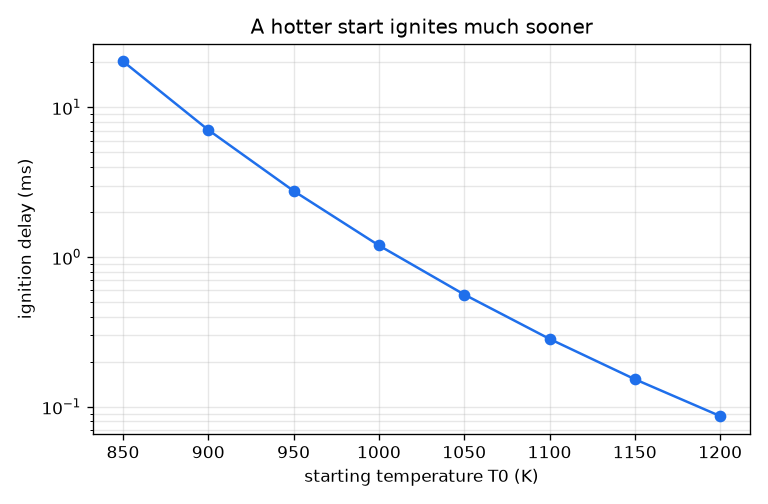
\includegraphics[width=0.85\linewidth]{figures/s01_delay_vs_start.png}\\\small The ignition delay (log scale) falls steeply with the start temperature.\end{center}

\subsection*{E. Worked example}
At a start temperature of 1000 K, find the rate constant k. If there were no heat feedback, how much fuel would be gone after 1 ms? Compare with the fuel burnt at the moment of ignition when the feedback is on.
\begin{enumerate}[nosep]
\item Ea / (R T) = 150000 / (8.314 * 1000) = 18.04.
\item k = 2.5e9 * exp(-18.04) = 36.5 per second.
\item Without feedback the temperature stays at 1000 K, so after 1 ms c = exp(-36.5 * 0.001) = exp(-0.0365) = 0.964: only 3.6 percent of the fuel is gone.
\item With feedback, ignition means T has risen by 400 K. Burning all the fuel would give 1500 K, so 400 K means a fraction 400 / 1500 = 0.267 of the fuel is burnt: 26.7 percent.
\item The simulation gives the ignition delay at 1000 K as 1.19 ms.
\end{enumerate}
\textbf{Answer.} k = 36.5 per second. With feedback off only 3.6 percent of the fuel burns in 1 ms; with feedback on, 26.7 percent has burnt when ignition is reached, after 1.19 ms.

\subsection*{F. Questions}
\begin{enumerate}[nosep]
\item \textbf{Conceptual.} Why does the mixture wait for a long time and then ignite almost instantly, even though the chemistry is the same all the time? Why does the box without heat feedback never ignite?
\item \textbf{Numerical.} Find the rate constant at 1100 K. By what factor is it bigger than at 1000 K? If 10 percent of the fuel burns, by how many kelvin does the box heat up?
\item \textbf{Graph and simulation interpretation.} In the right-hand figure, by what factor does the delay shrink when the start temperature rises from 1000 K to 1050 K? What does the steepness of the curve tell you about the rate?
\item \textbf{Design and optimisation challenge.} Design: you need ignition within 0.5 ms. Find the lowest start temperature (in steps of 10 K) that works with a heat release of 1500 K. Then find out whether a richer mixture with 2000 K heat release lets you start cooler, and say what you give up.
\end{enumerate}

\section{Session 2: The one-step model and the ignition-delay law}

\subsection*{A. Real-world problem}
An engine designer asks: how hot must the charge be so that it ignites within 1 millisecond, and what happens to the delay if the charge is 50 K cooler? In Session 1 we ran simulations and looked up answers; now we turn the model into equations we can solve and invert. The model is still a one-step toy with made-up numbers, for learning only: it keeps the part that all thermal ignition has in common (heat feedback on an Arrhenius rate) and leaves out chain branching, which dominates real hydrogen-oxygen ignition and gives it explosion limits. Never use it to design real equipment.

\subsection*{B. Concept and theory}
The model is dc/dt = -k c and dT/dt = DT\_AD k c for a lumped, insulated box at constant pressure with constant heat capacity cp, where DT\_AD = Q / cp is the heat released per unit fuel divided by cp. Dividing the two equations gives dT/dc = -DT\_AD, so T = T0 + DT\_AD (1 - c) at every instant: temperature and fuel are tied together. Substituting, the system collapses into one equation for c, and the time to go from c = 1 down to c* = 1 - 400 / DT\_AD (the point where T has risen by 400 K) is an integral, tau = integral of dc / (k c) from c* to 1, which we evaluate by Gauss-Legendre quadrature (no time stepping). The textbook estimate of Frank-Kamenetskii replaces k(T) by k(T0) exp(Ea (T - T0) / (R T0\textasciicircum{}2)), which gives tau = R T0\textasciicircum{}2 / (Ea DT\_AD k(T0)); it is a good guide but, because the true k grows more slowly than that exponential over a 400 K rise, it comes out too short. Over a range of start temperatures, ln(tau) plotted against 1000/T0 is nearly a straight line; a least-squares fit gives its slope, which is below Ea / (1000 R) because the gas heats up during the delay.

\begin{itemize}[nosep]
\item c: fuel left (1 = all) (no unit)
\item T0: start temperature (K)
\item DT\_AD: Q / cp, temperature rise if all fuel burns (1500) (K)
\item k(T): Arrhenius rate constant A exp(-Ea/(R T)), A = 2.5e9 1/s, Ea = 150 kJ/mol (1/s)
\item tau: ignition delay: time to reach T0 + 400 K (s)
\item Q: heat released per unit mass of fuel burnt (J/kg)
\item cp: specific heat of the gas (constant) (J/(kg K))
\end{itemize}

\begin{equation*}
\frac{dc}{dt}=-k(T)\,c,\qquad \frac{dT}{dt}=\Delta T_{ad}\,k(T)\,c,\qquad \Delta T_{ad}=\frac{Q}{c_p}
\end{equation*}

\begin{equation*}
\frac{dT}{dc}=-\Delta T_{ad}\;\Rightarrow\; T=T_0+\Delta T_{ad}\,(1-c)
\end{equation*}

\begin{equation*}
\tau=\int_{c^*}^{1}\frac{dc}{k\big(T_0+\Delta T_{ad}(1-c)\big)\,c},\qquad c^*=1-\frac{400\,\mathrm{K}}{\Delta T_{ad}}
\end{equation*}

\begin{equation*}
\tau_{FK}=\frac{R\,T_0^{2}}{E_a\,\Delta T_{ad}\,k(T_0)}
\end{equation*}

\begin{equation*}
\ln\tau\approx a+b\,\frac{1000}{T_0}
\end{equation*}

\begin{center}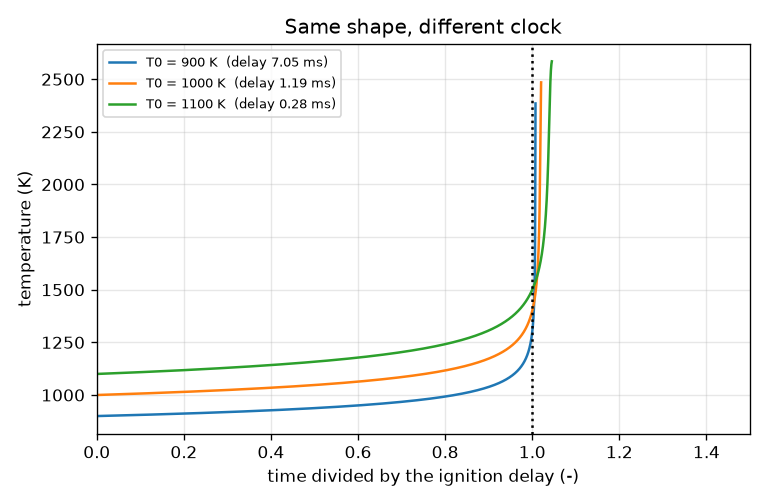
\includegraphics[width=0.85\linewidth]{figures/s02_curves_scaled.png}\\\small Temperature against time divided by the delay: same shape, different clock.\end{center}

\subsection*{E. Worked example}
For T0 = 1000 K, estimate the delay with the Frank-Kamenetskii formula by hand, and compare it with the integral computed by the code.
\begin{enumerate}[nosep]
\item k(T0) = 2.5e9 * exp(-18.04) = 36.514 per second (Session 1).
\item R T0\textasciicircum{}2 = 8.314 * 1 000 000 = 8.314e6 J/mol.
\item Ea DT\_AD k(T0) = 150000 * 1500 * 36.514 = 8.216e9 J/mol per second.
\item tau\_FK = 8.314e6 / 8.216e9 = 1.012e-3 s = 1.01 ms.
\item The integral evaluated by the code gives 1.192 ms, so the estimate is 0.849 (85 percent) of it.
\end{enumerate}
\textbf{Answer.} The estimate gives 1.01 ms and the integral 1.19 ms: the textbook formula is about 15 percent too short at 1000 K, because the true rate grows more slowly than the exponential it assumes.

\subsection*{F. Questions}
\begin{enumerate}[nosep]
\item \textbf{Conceptual.} Why is ln(delay) against 1000/T0 nearly a straight line, and why is its slope smaller than Ea / (1000 R)?
\item \textbf{Numerical.} Use the Frank-Kamenetskii formula by hand to estimate the delay at 1100 K, and compare it with the exact value 0.2829 ms.
\item \textbf{Graph and simulation interpretation.} From the ln(delay) plot, read the slope between the points at 900 K and 1100 K. Is it equal to the fitted slope 15.96? Why can it differ?
\item \textbf{Design and optimisation challenge.} Design: the charge can only be heated to 950 K, but you need a 1 ms delay. Using a catalyst-like additive that multiplies the pre-exponential factor A, by what factor must A grow? Name one other lever and its cost.
\end{enumerate}

\section{Session 3: Stiffness: explicit versus implicit, and how to trust the answer}

\subsection*{A. Real-world problem}
Combustion codes spend most of their time on ignition-type chemistry because it is stiff: for a long time almost nothing changes, then everything changes within microseconds, and afterwards a very fast mode remains that must be integrated stably. How do we compute the delay reliably, how much does each method cost, and how do we know the answer is right? The model is still the one-step toy of Sessions 1 and 2, with made-up numbers; real hydrogen-oxygen ignition is a chain-branching network with explosion limits that are not in this toy, and nothing here is a validated design tool.

\subsection*{B. Concept and theory}
Write the state as y = (T, c) with dy/dt = f(y). The Jacobian J = df/dy (a 2x2 matrix) has eigenvalues that are the time scales of the model: after ignition c is almost zero and one eigenvalue is about -k(T\_final), a decay of millions per second. An explicit method such as RK4 (four right-hand-side evaluations per step, no solving) is stable only if step times the fastest decay rate is below about 2.785, so the step is limited by stability, not by accuracy, long after ignition has finished. An implicit method defines the new state by an equation containing itself, for example the trapezoid rule z = y + h/2 (f(y) + f(z)), solved by Newton iteration with the Jacobian; it costs a 2x2 linear solve per iteration but is stable for large steps. Adaptive steps compare one full step with two half steps to estimate the local error. We validate with the exact quadrature of Session 2, with the analytic Semenov criterion (heat loss h to surroundings at Ta, fuel held constant: a steady state exists only if psi = DT\_AD k(Ta) Ea / (R Ta\textasciicircum{}2 h) is at most 1/e), and with the normalised sensitivity S\_x = d ln tau / d ln x. For pressure we use the illustrative rule k proportional to (P/P0)\textasciicircum{}m with m = 1; real behaviour is not a simple power law.

\begin{itemize}[nosep]
\item y = (T, c): state: temperature and fuel left (K, no unit)
\item J: Jacobian df/dy, 2x2 (1/s)
\item h (step): time step of an integrator (s)
\item h (loss): heat-loss rate to the surroundings (1/s)
\item Ta: surrounding temperature in the Semenov test (K)
\item psi: Semenov parameter; critical value 1/e (no unit)
\item S\_x: normalised sensitivity d ln tau / d ln x (no unit)
\item m: toy pressure exponent (1) (no unit)
\item rtol: relative tolerance of the adaptive solvers (no unit)
\end{itemize}

\begin{equation*}
\dot T=\Delta T_{ad}\,k(T)\,c-h\,(T-T_a),\qquad \dot c=-k(T)\,c
\end{equation*}

\begin{equation*}
J=\begin{pmatrix}\Delta T_{ad}\,k'\,c-h & \Delta T_{ad}\,k\\ -k'\,c & -k\end{pmatrix},\qquad k'=k\,\frac{E_a}{RT^2}
\end{equation*}

\begin{equation*}
\text{RK4 stable only if } h\,|\lambda|\lesssim 2.785,\quad |\lambda|\approx k(T_0+\Delta T_{ad})
\end{equation*}

\begin{equation*}
z=y+\tfrac{h}{2}\big(f(y)+f(z)\big)\quad\text{(trapezoid; Newton: } (I-\tfrac{h}{2}J)\,\delta=-g\text{)}
\end{equation*}

\begin{equation*}
\psi=\frac{\Delta T_{ad}\,k(T_a)\,E_a}{R\,T_a^{2}\,h}\le \frac1e\ \text{ for a steady state}
\end{equation*}

\begin{equation*}
S_x=\frac{d\ln\tau}{d\ln x},\qquad \tau\propto P^{-m}
\end{equation*}

\begin{center}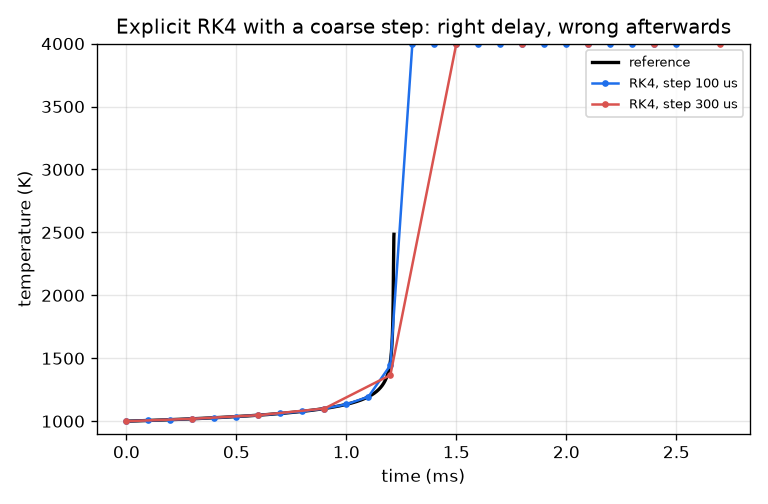
\includegraphics[width=0.85\linewidth]{figures/s03_coarse_step_failure.png}\\\small Explicit RK4 with 100 and 300 microsecond steps: the delay is almost right, the state afterwards is wrong.\end{center}

\subsection*{E. Worked example}
For T0 = 1000 K find the fast decay rate after ignition and the largest stable RK4 step. Then check it by running RK4 just below and just above that step.
\begin{enumerate}[nosep]
\item After ignition T = 1000 + 1500 = 2500 K and c is almost zero, so the fastest eigenvalue of the Jacobian is about -k(2500 K).
\item Ea / (R T) = 150000 / (8.314 * 2500) = 7.217, exp(-7.217) = 7.34e-4, so k = 2.5e9 * 7.34e-4 = 1.84e6 per second.
\item The RK4 stability limit is 2.785 / 1.84e6 = 1.52e-6 s = 1.52 microseconds.
\item RK4 with a step of 1.45 microseconds ends correctly at 2500 K with the fuel gone.
\item RK4 with 1.6 microseconds stays finite but ends wrong (the temperature is below 2450 K and more than 5 percent of the fuel is left); with 5 microseconds it blows up, even though the delay it found before the blow-up is right to 0.01 percent.
\end{enumerate}
\textbf{Answer.} The fast decay rate is 1.84e6 per second and the RK4 step limit is 1.52 microseconds: the accurate ignition event is found with big steps, but covering the time after ignition explicitly forces steps hundreds of times smaller than the delay itself (1.19 ms).

\subsection*{F. Questions}
\begin{enumerate}[nosep]
\item \textbf{Conceptual.} Why must an explicit method keep taking microsecond steps after the ignition is over, when the temperature is no longer changing? Why can an implicit method take huge steps there?
\item \textbf{Numerical.} For a run started at 900 K, find the final temperature, the decay rate k(final T) and the RK4 stability limit.
\item \textbf{Graph and simulation interpretation.} In the steps-against-tolerance figure, why is the RK4 curve flat while the trapezoid curve rises? What does that mean for the choice of solver at a loose or a tight tolerance?
\item \textbf{Design and optimisation challenge.} Design: you must compute the delay to within 0.1 percent for a large number of cells over 30 ms each. Which solver and tolerance do you choose, and how much does it save? State the assumption.
\end{enumerate}

\section{Real-world mini-project}
\textbf{Tabulate the ignition delay of a toy fuel and draw its law.} A new toy fuel B has the made-up numbers A = 1e7 per second, Ea = 110 kJ/mol and a heat release of 1200 K (stored as \texttt{FUEL\_B} in the Session 3 lesson). Using the adaptive implicit solver \texttt{trapezoid\_adaptive} (through \texttt{delay\_table}), tabulate its ignition delay for start temperatures from 800 K to 1300 K in steps of 50 K, compare each value with the exact quadrature \texttt{reference\_delay}, draw ln(delay) against 1000/T0 with a straight-line fit, and read off the start temperature that gives a 1 ms delay.

\section{The path ahead}
\begin{enumerate}[nosep]
\item \textbf{Session 4: A chain-branching toy with an explosion limit.} A three-variable toy (fuel, a radical pool, temperature) whose delay depends on pressure in a non-monotone way.
\item \textbf{Session 5: Variable heat capacity.} A reactor with a temperature-dependent cp (a simple polynomial) in place of the constant DT\_AD.
\item \textbf{Session 6: A higher-order stiff solver.} An implicit solver of order three or more with an analytic Jacobian.
\item \textbf{Session 7: Include fuel burn-up in the Semenov boundary.} A modified criterion or a quick numerical correction for the critical surrounding temperature.
\item \textbf{Session 8: Hot-spot ignition in one dimension.} A one-dimensional grid with heat conduction added to the toy reaction.
\end{enumerate}

\section{Answers and hints}

\subsection*{Session 1}
\begin{enumerate}[nosep]
\item \textbf{Conceptual.} Hint: Think about what the temperature does to the rate, and what the rate does to the temperature. Solution: The rate k grows steeply with temperature and the reaction heats the gas, so the process feeds itself: a positive feedback loop (thermal runaway). While little fuel has burnt the heating is tiny, so the temperature and the rate barely change and the gas seems to wait; once the temperature has risen enough, each increment of heat makes the rate noticeably larger and the loop accelerates until the fuel is gone. Without feedback the temperature stays at its start value, the rate stays constant and the fuel simply decays slowly (3.6 percent in 1 ms), so there is no runaway.
\item \textbf{Numerical.} Hint: Ea / (R T) at 1100 K, then exp of minus that; heat = fraction burnt times DT\_AD. Solution: Ea / (R T) = 150000 / (8.314 * 1100) = 16.40, so k = 2.5e9 * exp(-16.40) = 188 per second. The factor is 188 / 36.5 = 5.2. A 10 percent burn heats the box by 0.1 * 1500 = 150 K. Sanity check: a hotter gas must have a larger k, and a small fraction of fuel burnt gives a small fraction of 1500 K.
\item \textbf{Graph and simulation interpretation.} Hint: Read the delay at both temperatures and divide; the delay is on a log scale. Solution: The delay falls from about 1.2 ms to about 0.56 ms, a factor of about 2.1. A modest 50 K change halves the wait, because k itself changes steeply with temperature (k is 5.2 times larger at 1100 K than at 1000 K), so the runaway starts sooner.
\item \textbf{Design and optimisation challenge.} Hint: Use euler\_delay(T0) for T0 = 1050, 1060, ... and then euler\_delay(T0, 2000.0). Solution: At 1050 K the delay is 0.562 ms (too slow); at 1060 K it is 0.488 ms, so the lowest start temperature is 1060 K. With a 2000 K heat release the delay at 1050 K is 0.416 ms, so a richer mixture works from 1050 K, 10 K cooler (and from lower still). Trade-off: a richer mixture means more fuel per air, so a hotter burnt gas (2000 K above the start) and, in a real engine, more emissions and a greater risk of knock; a hotter start needs a higher compression. This is a toy: it only shows the direction of the trade-off.
\end{enumerate}

\subsection*{Session 2}
\begin{enumerate}[nosep]
\item \textbf{Conceptual.} Hint: Think of a rate proportional to exp(-Ea/(R T)) and of what the gas temperature does during the delay. Solution: The delay is roughly the reciprocal of a rate that depends on T0 through exp(-Ea/(R T0)), so ln(delay) is roughly linear in 1/T0 with slope Ea/R (per unit 1/T0, or Ea/(1000 R) per unit 1000/T0). But during the delay the gas heats by 400 K, so most of the wait is spent at temperatures above T0, where the rate is higher and the dependence on T0 is weaker; that lowers the effective slope (15.96 instead of 18.04).
\item \textbf{Numerical.} Hint: k(1100 K) = 188.3 per second from Session 1; tau = R T0\textasciicircum{}2 / (Ea DT\_AD k). Solution: R T0\textasciicircum{}2 = 8.314 * 1.21e6 = 1.006e7. Ea DT\_AD k = 150000 * 1500 * 188.27 = 4.236e10. tau\_FK = 1.006e7 / 4.236e10 = 2.375e-4 s = 0.2375 ms, which is 0.84 of the exact 0.2829 ms. Sanity check: shorter than at 1000 K (1.01 ms), as it must be.
\item \textbf{Graph and simulation interpretation.} Hint: Slope = change in ln(delay) divided by change in 1000/T0, using ln(7.0495e-3) = -4.955 and ln(0.2829e-3) = -8.171. Solution: The slope is (-4.955 + 8.171) / (1000/900 - 1000/1100) = 3.216 / 0.202 = 15.9, close to but not exactly the fit value 15.96: the points are not on a perfectly straight line (R squared is 0.99996, not 1), and the local slope is slightly different from place to place.
\item \textbf{Design and optimisation challenge.} Hint: Doubling A halves the delay exactly. Find the delay at 950 K first. Solution: The delay at 950 K is 2.759 ms, so A must grow by 2.759 / 1.0 = 2.76 times. Another lever is a richer mixture (a larger DT\_AD), which shortens the delay, or a lower activation energy; the cost of a richer mixture is more fuel, a hotter burnt gas and more emissions. Assumption: the toy keeps the same law with a larger A, which a real additive would not do exactly.
\end{enumerate}

\subsection*{Session 3}
\begin{enumerate}[nosep]
\item \textbf{Conceptual.} Hint: Think of the fast decaying mode of the Jacobian and of what a stability limit is. Solution: After ignition the fuel is almost zero and a very fast mode, decaying at about k(T\_final) per second, remains. Any error in that mode is damped in reality, but an explicit method amplifies it if step times decay rate exceeds about 2.785, so the step must be below a stability limit of about 1.5 microseconds even though the solution itself is flat. An implicit method evaluates the right-hand side at the new state, so the fast decay is damped for any step size; it needs only enough accuracy for the slow behaviour.
\item \textbf{Numerical.} Hint: Final T = T0 + 1500; limit = 2.785 / k. Solution: Final T = 900 + 1500 = 2400 K. Ea / (R T) = 150000 / (8.314 * 2400) = 7.517, so k = 2.5e9 * exp(-7.517) = 1.36e6 per second. The limit is 2.785 / 1.36e6 = 2.05 microseconds, a little larger than at 1000 K because the final temperature is lower.
\item \textbf{Graph and simulation interpretation.} Hint: Which limit sets the RK4 step: accuracy or stability? Solution: The RK4 step is set by stability, so tightening the tolerance barely changes it (the step counts stay within 6 percent from 1e-2 to 1e-6). The trapezoid step is set by accuracy, so its step count grows by more than 7 times over the same range, but it stays far below RK4's at all of these tolerances for this stiff problem. If the tolerance were very tight and the problem not stiff, the explicit method could win; for stiff chemistry the implicit method is the right default.
\item \textbf{Design and optimisation challenge.} Hint: Compare the number of right-hand-side calls and the delay error at tolerance 1e-3 for both solvers. Solution: At tolerance 1e-3 the adaptive trapezoid gives a delay within 0.1 percent using fewer than 2000 right-hand-side calls, while RK4 needs more than 100 times as many. So choose the implicit solver with tolerance 1e-3. Assumption: the Jacobian is cheap (2x2 here); in a real mechanism with many species the Jacobian and linear solve cost more, which reduces but usually does not remove the advantage.
\end{enumerate}

\section{How to join}
Read \texttt{CONTRIBUTING.md} in the repository, then pick an issue labelled \texttt{good first issue}. Repository: \url{https://github.com/KrunalPanchal1995/pan-iit-oss/tree/main/openignition}

\end{document}
